\section{Theory of GAN}

\subsection{Math Idea}
生成问题本质是极大似然估计; 现有真实数据$P_{data}(x)$, 生成器生成的数据为$P_{G}(x;\theta)$, 我们希望$P_{G}(x;\theta)$更加接近$P_{data}(x)$. 从真实数据$P_{data}(x)$中取样${x^{1}, x^{2},... ,x^{m}}$, 可计算出$P_{G}(x^{i};\theta)$, 希望能找到参数$\theta^{\star}$使$L=\prod_{i=1}^{m}P_{G}(x^{i};\theta)$最大.

% \begin{equation*}
%     \theta^{\star} = arg \max \limits_{\theta} \prod_{i=1}^{m} P_{G}(x^{i};\theta)
% \end{equation*}

\begin{align*}
    \theta^{\star} & = arg \max \limits_{\theta} \prod_{i=1}^{m} P_{G}(x^{i};\theta) \\
    & = arg \max \limits_{\theta} log\sum_{i=1}^{m} P_{G}(x^{i};\theta)  \\
    & = arg \max \limits_{\theta} \sum_{i=1}^{m} log P_{G}(x^{i};\theta)  \\
    & \approx arg \max \limits_{\theta} E_{x\sim P_{data}}[logP_{G}(x;\theta)] \\
    & = arg \max \limits_{\theta} \int_{x} P_{data}(x)logP_{G}(x;\theta) dx - \int_{x} P_{data}(x)logP_{data}(x) dx \\
    & = arg \max \limits_{\theta} \int_{x} P_{data}(x)(logP_{G}(x;\theta) - logP_{data}(x)) dx\\
    & = arg \max \limits_{\theta} \int_{x} P_{data}(x)log \frac{P_{G}(x;\theta)}{P_{data}(x)} dx\\
    & = arg \min \limits_{\theta} KL(P_{data}\parallel P_{G})
\end{align*}

KL离散度可表示为两个分布之间的差异, 定义为:
\begin{equation*}
    D_{KL}(p\parallel q) = -\sum_{x}p(x)log\frac{q(x)}{p(x)}
\end{equation*}

因此generate这个问题的数学本质是在让生成数据的分布更加贴近真实数据的分布来达到以假乱真的目的. 

\subsection{Generator}
训练生成器的目的是使生成数据分布与真实数据分布差异最小, 即优化下式:
\begin{equation*}
    G^{\star} =  arg \min \limits_{G} Div(P_{G}, P_{data})
\end{equation*}
如果已知$P_{G}, P_{data}$的分布, 直接使用梯度下降则可求解, 但现在问题是两者的分布未知. 而且分布较为复杂, 因为在深度学习之前的方法, 由于网络较浅, 无法模拟复杂的分布, 导致其生成效果不佳. 

\subsection{Discriminator}
对于上述问题, GAN的数学思想是, 通过对$P_{G}, P_{data}$的采样, 来估计两者分布, 通过Discriminator来评判两者分布的差异, 即通过最大化$V(G,D)$:

\begin{align*}
    V &= E_{x\sim P_{data}}(logD(x)) + E_{x\sim P_{G}}( log(1-D(x))) \\
    & = \int_{x} P_{data}(x) logD(x) dx + \int_{x} P_{G}(x) log(1-D(x)) dx \\
    & = \int_{x}(P_{data}(x) logD(x) + P_{G}(x) log(1-D(x))) dx
\end{align*}

假设$D(x)$可以表示任意函数, 则对上式求最大值则为对$P_{data}(x) logD(x) + P_{G}(x) log(1-D(x))$求最大值, 如式:

\begin{equation*}
    f(D) = a \cdot log(D) + b \cdot log(1-D) 
\end{equation*}
其中$a = P_{data}(x)$, $b = P_{G}(x)$, 则通过求导可得
\begin{align*}
    D^{\star} &= \frac{a}{a+b} \\
    & = \frac{P_{data}(x)}{P_{data}(x) + P_{G}(x)}
\end{align*}

将$D^{\star}$带入$V$, 可得:
\begin{align*}
    \max \limits_{D} V(G,D) &= V(G, D^{\star}) \\
    & =  E_{x\sim P_{data}}(log\frac{P_{data}(x)}{P_{data}(x) + P_{G}(x)}) + E_{x\sim P_{G}}(\frac{P_{G}(x)}{P_{data}(x) + P_{G}(x)}) \\
    & = -2log(2) \\
    & + E_{x\sim P_{data}}(log\frac{P_{data}(x)}{(P_{data}(x) + P_{G}(x))/2}) + E_{x\sim P_{G}}(\frac{P_{G}(x)}{(P_{data}(x) + P_{G}(x))/2}) \\
    & = -2log(2) \\
    & + \int_{x} P_{data}(x) log(\frac{P_{data}(x)}{(P_{data}(x) + P_{G}(x))/2}) + \int_{x} P_{G}(x) log(\frac{P_{G}(x)}{(P_{data}(x) + P_{G}(x))/2}) \\
    & = -2log(2) + KL(P_{data}\parallel \frac{P_{data}+P_{G}}{2} ) + KL(P_{G}\parallel \frac{P_{data}+P_{G}}{2})\\
    & = -2log(2) + 2JSD(P_{data}\parallel P_{G})
\end{align*}

JS离散度表示两个分布的相似性. 也就是通过Discriminator通过打分的表象其本质也是在求两个分布的相似性. 


% ((P_{data}\parallel \frac{P_{data}+P_{G}}{2} ))
\subsection{Conclusion}
通过GAN将$G^{\star} = arg \min \limits_{G} Div(P_{G}, P_{data})$, $D^{\star} = arg \max \limits_{D} V(D,G)$, 转换成了$G^{\star} = arg \min \limits_{G} \max \limits_{D} V(G, D)$. 

\begin{figure}[!htbp]
    \centering
    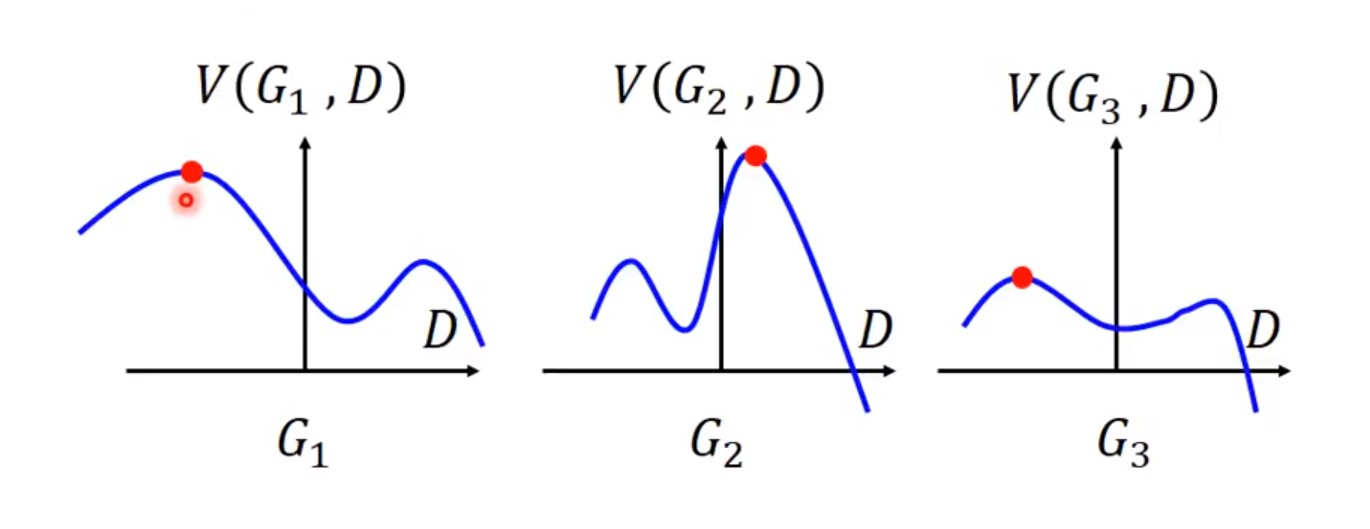
\includegraphics[height=10em]{pic/pic0302.jpg}
    \caption{测试}
    \label{fig:0302}
\end{figure}


如图~\ref{fig:0301}论文中图所示, 其训练过程为两个分布渐渐相似. 
\begin{figure}[!htbp]
    \centering
    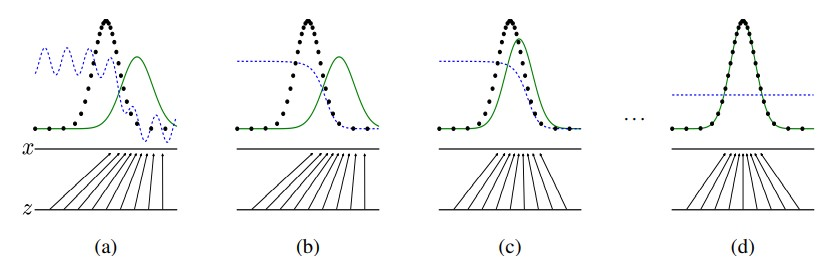
\includegraphics[height=10em]{pic/pic0301.jpg}
    \caption{训练过程}
    \label{fig:0301}
\end{figure}

但要注意每一次训练迭代时, G和D的步长和次数.



